\documentclass[tikz, border=25pt]{standalone}
\usetikzlibrary{shapes.geometric, arrows.meta, positioning, fit, backgrounds, calc}

\begin{document}
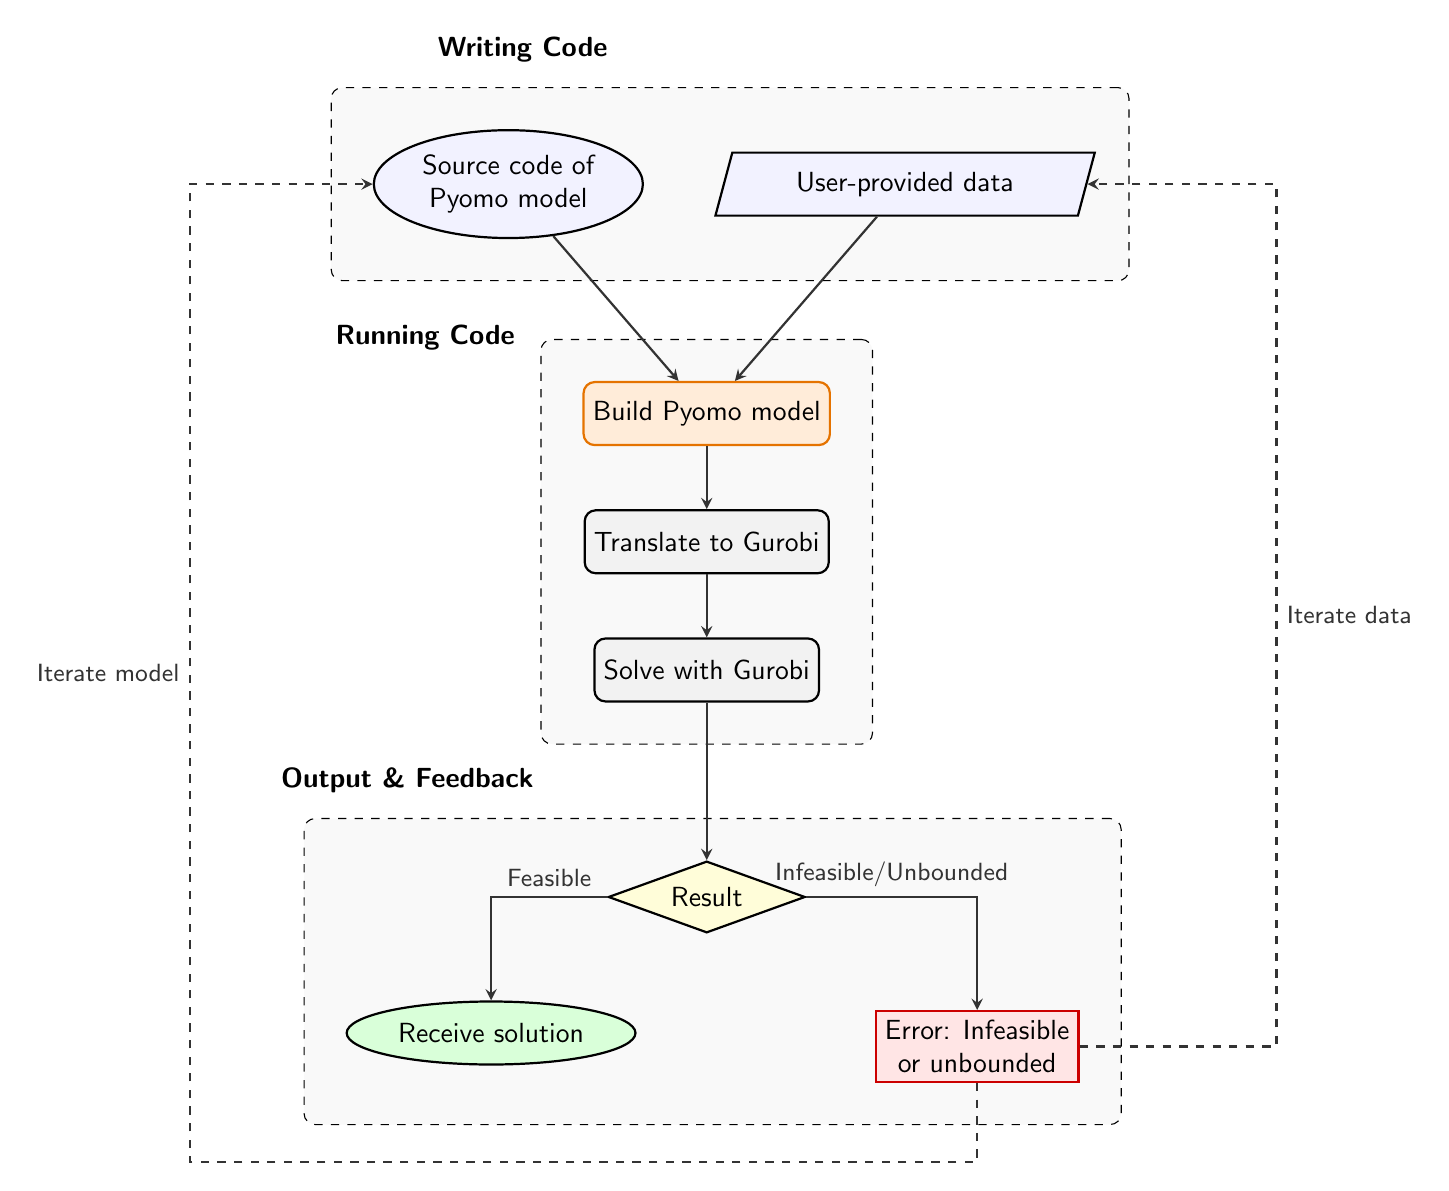
\begin{tikzpicture}[
    % --- Global Styles ---
    base/.style={draw, thick, align=center, minimum height=0.8cm, minimum width=2.5cm, font=\sffamily},
    data/.style={base, trapezium, trapezium left angle=75, trapezium right angle=105, fill=blue!5},
    source/.style={base, ellipse, fill=blue!5},
    process/.style={base, rectangle, rounded corners, fill=gray!10},
    % Changed the bottleneck to Orange to distinguish it from the Red error state
    bottleneck/.style={process, fill=orange!15, draw=orange!90!black, thick}, 
    decision/.style={base, diamond, fill=yellow!15, aspect=2, inner sep=2pt},
    success/.style={base, ellipse, fill=green!15},
    error/.style={base, rectangle, fill=red!10, draw=red!80!black},
    container/.style={draw, dashed, rounded corners, inner sep=15pt, fill=gray!5},
    arrow/.style={->, >=stealth, thick, color=black!80},
    dashed arrow/.style={->, >=stealth, thick, dashed, color=black!80}
]

    % --- Nodes & Absolute Positioning ---
    
    \node[source] (source) {Source code of\\Pyomo model};
    \node[data, right=1.0cm of source] (data) {User-provided data};

    \node[bottleneck, below=2.5cm of $(source)!0.5!(data)$] (build) {Build Pyomo model};
    \node[process, below=0.8cm of build] (translate) {Translate to Gurobi};
    \node[process, below=0.8cm of translate] (solve) {Solve with Gurobi};

    \node[decision, below=2cm of solve] (feedback) {Result};
    \node[success, below left=1.2cm and 0.8cm of feedback] (sol) {Receive solution};
    \node[error, below right=1.2cm and 1.5cm of feedback] (nosol) {Error: Infeasible\\or unbounded};

    % --- Subgraph Bounding Boxes ---
    % yshift added to ensure the label sits slightly above the dashed line
    \begin{scope}[on background layer]
        \node[container, fit=(source)(data), label={[font=\sffamily\bfseries, xshift=-2mm, yshift=2mm]above left:Writing Code}] (writing) {};
        \node[container, fit=(build)(translate)(solve), label={[font=\sffamily\bfseries, xshift=-2mm, yshift=2mm]above left:Running Code}] (running) {};
        \node[container, fit=(feedback)(sol)(nosol), label={[font=\sffamily\bfseries, xshift=-2mm, yshift=2mm]above left:Output \& Feedback}] (output) {};
    \end{scope}

    % --- Forward Flow Logic ---
    \draw[arrow] (source) -- (build);
    \draw[arrow] (data) -- (build);
    \draw[arrow] (build) -- (translate);
    \draw[arrow] (translate) -- (solve);
    \draw[arrow] (solve) -- (feedback);
    
    \draw[arrow] (feedback) -| node[above, near start, font=\sffamily\small] {Feasible} (sol);
    \draw[arrow] (feedback) -| node[above, near start, font=\sffamily\small] {Infeasible/Unbounded} (nosol);

    % --- Explicit Feedback Loops ---
    
    % Route 1: Out the right, pushed 2.5cm wide. Label moved to the vertical climb (pos=0.25).
    \draw[dashed arrow] (nosol.east) -- ++(2.5,0) |- node[pos=0.25, right, font=\sffamily\small] {Iterate data} (data.east);
    
    % Route 2: Out the bottom, dropped 1cm down, swept 10cm left. Label moved to the vertical climb (pos=0.25).
    \draw[dashed arrow] (nosol.south) -- ++(0,-1.0) -| ++(-10,0) |- node[pos=0.25, left, font=\sffamily\small] {Iterate model} (source.west);

\end{tikzpicture}
\end{document}